




\section{Power system of Railway Transportation System}


In this section is started the literature review of this document, with the coverage of the power system of \ac{RTS}. This system is reported in 2013 to transport 6.4\% transport modal share of people and 8.7\% transport modal share of goods, \cite{iea-uic2016}. With high influence in the transportation of goods and people in the last century, this system had substantial technological enhancements. Currently we have a \ac{RTS} with substantial differences in the supply system.

In subsection \ref{subs:311} is presented an overview on European railway electrical supply systems. Later on, in subsection \ref{subs:312}, a comparison between different catenary supply systems is presented and in subsection \ref{subs:313} is presented a comparison of the power system architecture of trains. A further detail on train electrical components is presented in subsection \ref{subs:314}.

This section is supported on the chapter 5 of the work of \cite{abad2016}. Further reading of this book chapter is recommended. 

\subsection{Overview of Existing European Railway Power Systems}
\label{subs:311}
Back to the 19th century, the steam turbine was the main propulsion system for the trains. Later on, electric and diesel propulsion systems were adopted. In recent years occurred a massive introduction of power converters based on \ac{IGBT}, which allowed an increase of energy efficiency (allowing, for example, regenerative breaking and reduction of power losses in traction motors).

Due to this evolution, different topologies of the railway system exists nowadays. In table \ref{tab:31.t1}, different catenary topologies are visible which results in different power systems for \ac{RTS}.


% Table generated by Excel2LaTeX from sheet 'Sheet1'
\begin{table}[htbp]
	\centering
	\tiny
	\caption{Catenary topology and vehicle characteristics of different railway vehicles. \cite{abad2016}.}
	\begin{tabular}{|c|p{10.145em}p{10.355em}|cc|}
		\cmidrule{2-5}    \multicolumn{1}{c|}{} & \multicolumn{2}{c|}{\textbf{Catenary topology}} & \multicolumn{2}{c|}{\textbf{Vehicle characteristics}} \\
		\cmidrule{2-5}    \multicolumn{1}{c|}{} & \multicolumn{1}{c}{\textbf{DC supply}} & \multicolumn{1}{c|}{\textbf{AC supply}} & \textbf{Power} & \textbf{Top speed} \\
		\midrule
		\textbf{Tram} & 600V DC, 750V DC, 900V DC & \multicolumn{1}{c|}{-}     & 150–300kW & 50–70km/h \\
		\midrule
		\textbf{Metro} & 750V DC, 1500V DC & \multicolumn{1}{c|}{-}     & 350kW–1MW & 80km/h \\
		\midrule
		\textbf{Train} & 750V DC, 1500V DC, 3000V DC & 15kV AC (16.7Hz) and 25kV AC (50Hz) & 200kW–8MW & 120–350km/h \\
		\midrule
		\textbf{Locomotive} & 750V DC, 1500V DC, 3000V DC & 15kV AC (16.7Hz) and 25kV AC (50Hz) & 500kW–8MW & 100–200km/h \\
		\bottomrule
	\end{tabular}%
	\label{tab:31.t1}%
\end{table}%


Across the Europe, \ac{RTS} depends on different types of electrification systems, as it is illustrated in figure \ref{fig:abad2016}.


\begin{figure}[h!]
	\centering
	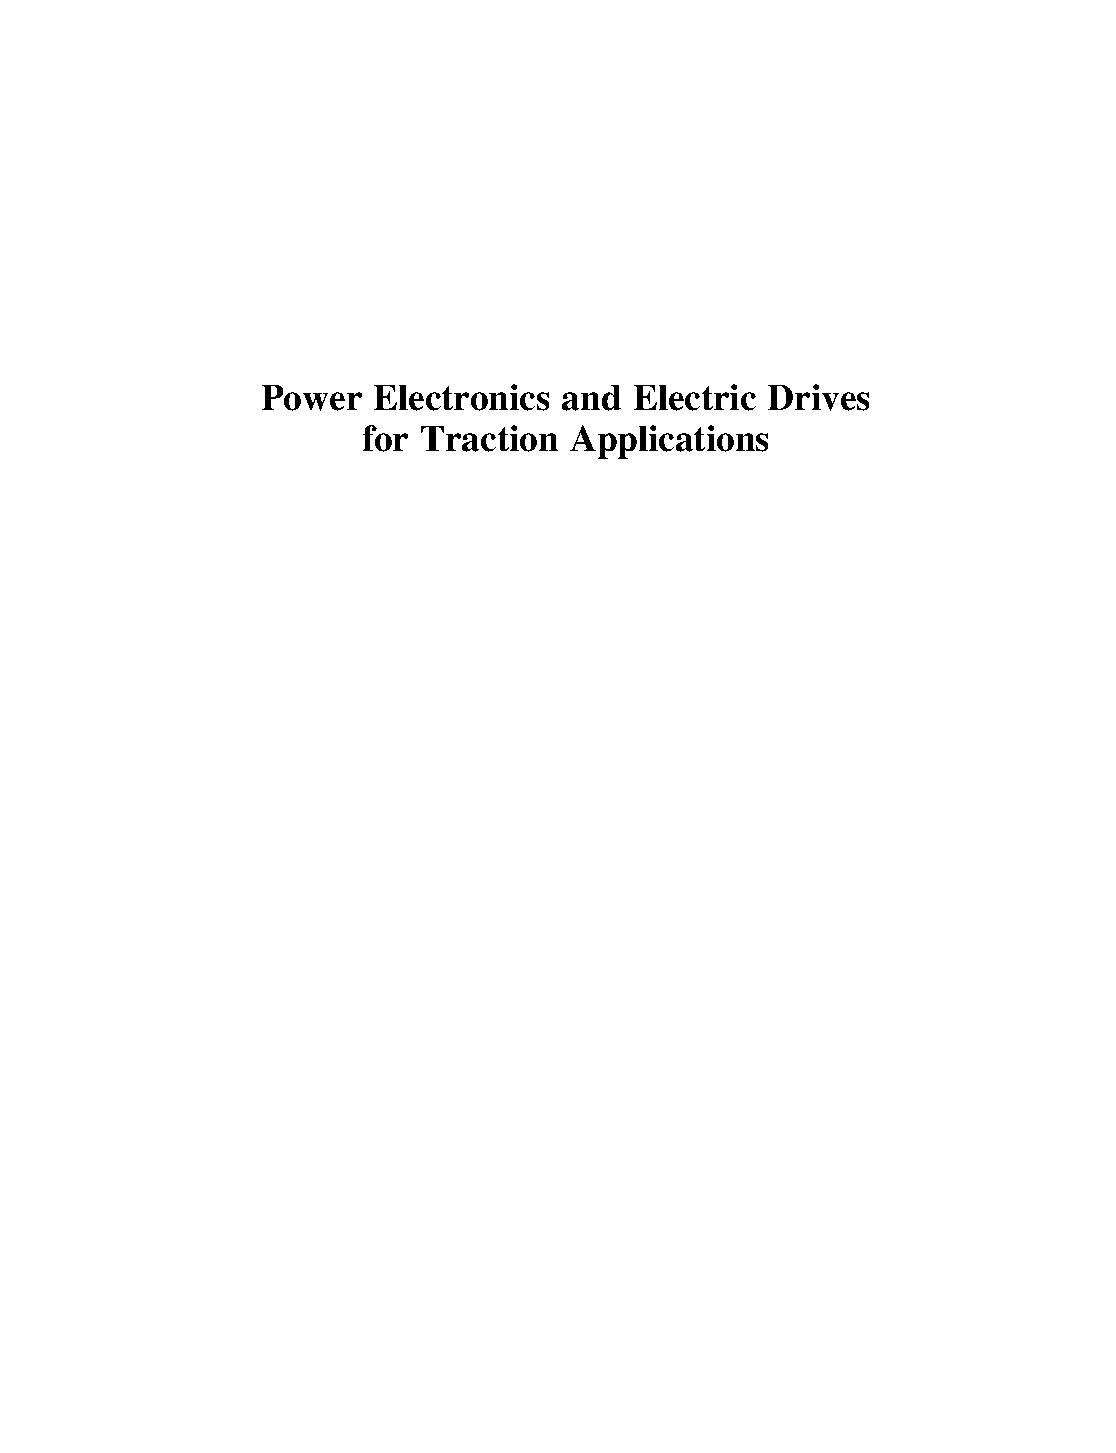
\includegraphics[width=0.7\textwidth,keepaspectratio]{figures/31.PowerS/abad2016}
	\caption{Railway main-line power supply systems in Europe. Adapted from \cite{abad2016}.}
	\label{fig:abad2016}
\end{figure}



\subsection{Railway Power Supply System}
\label{subs:312}

Similarly to the electrical grid, where a broad area of loads must be supplied, the railway power system must be capable of maintaining trains running in a broad area. The energy is supplied to the railway system through traction substations, similarly to the generation units of the electrical grid.

These traction substations ensure the interface between the electrical grid and the railway system, being responsible of supplying the distribution line of the railway system - or catenary.

As previously referred, the catenary can be divided in three main topologies:

%\begin{itemize}
%	\setlength\itemsep{-0.5em}
%	
%	\item DC supply system (six-, or 12-pulse diode rectifiers);
%	
%	\item AC 50Hz (or 60Hz) supply system;
%	
%	\item AC 16.7Hz supply system;
%
%\end{itemize}

\paragraph{$\bullet$ DC supply system\\}

The \ac{DC} supply system depends on rectifier converters (controlled or uncontrolled) and this railway power supply topology requires several traction substations, towards the reduction of power losses in catenary due to the high value of the electric current. In figure \ref{fig:abad2016f} is presented the supply architecture of such lines.

\begin{comment}
	\begin{figure}[h!]
	\centering
	\begin{minipage}{.5\textwidth}
	\centering
	%		\vspace{2.5em}
	\includegraphics[width=\textwidth,keepaspectratio]{figures/31.PowerS/abad2016b}
	%		\vspace{2em}
	\captionof{figure}{6-pulse and 12-pulse diode rectifier configurations. Adapted from \cite{abad2016}.}
	\label{fig:abad2016b}
	\end{minipage}%
	\begin{minipage}{.03\textwidth}  ~\end{minipage}	
	\begin{minipage}{.4\textwidth}
	\centering
	\includegraphics[width=\textwidth,keepaspectratio]{figures/31.PowerS/abad2016f}
	%		\vspace{0.5em}
	\captionof{figure}{DC supply system architecture. Adapted from \cite{abad2016}.}
	\label{fig:abad2016f}
	\end{minipage}
	\end{figure}
\end{comment}


\begin{figure}[h!]
	\centering
	\begin{minipage}{.7\textwidth}
		\centering
		\includegraphics[width=0.8\textwidth,keepaspectratio]{figures/31.PowerS/abad2016f}
		%		\vspace{0.5em}
		\captionof{figure}{\ac{DC} supply system architecture. Adapted from \cite{abad2016}.}
		\label{fig:abad2016f}
	\end{minipage}
\end{figure}




\paragraph{$\bullet$ AC 50Hz (or 60Hz) supply system\\}

With \ac{AC} catenaries, low frequency single-phase on-board transformer is required to step down the catenary voltage (25 kV or 15 kV) to the rectifier operating voltage (the rectifier is a single-phase voltage source converter, usually with bi-directional power flow).

On the traction substation, a special setup of power transformers avoids the usage of complete power converters. In figure \ref{fig:abad2016d} is presented the substation setup to supply a single-phase 50 Hz catenary.

\begin{figure}[h!]
	\centering
	\begin{minipage}{.7\textwidth}
		\centering
		\includegraphics[width=0.8\textwidth,keepaspectratio]{figures/31.PowerS/abad2016d}
		%		\vspace{0.5em}
		\captionof{figure}{50 Hz 25 kV supply system. Adapted from \cite{abad2016}.}
		\label{fig:abad2016d}
	\end{minipage}
\end{figure}


\paragraph{$\bullet$ AC 16.7 Hz supply systems\\}
An alternative setup is presented in figure \ref{fig:abad2016e} where a single-phase 16.7 Hz supply voltage is generated with a complete power converter. 
%\vspace{-2.5em}

\begin{figure}[h!]
	\centering
	\begin{minipage}{.7\textwidth}
		\centering
		\includegraphics[width=0.8\textwidth,keepaspectratio]{figures/31.PowerS/abad2016e}
		%		\vspace{0.5em}
		\captionof{figure}{16.7 Hz 15 kV supply system. Adapted from \cite{abad2016}.}
		\label{fig:abad2016e}
	\end{minipage}
\end{figure}

\begin{comment}
\begin{figure}[h!]
	\centering
	\begin{minipage}{.45\textwidth}
		\centering
		%		\vspace{2.5em}
		\includegraphics[width=\textwidth,keepaspectratio]{figures/31.PowerS/abad2016d}
		%		\vspace{2em}
		\captionof{figure}{50Hz 25kV supply system. Adapted from \cite{abad2016}.}
		\label{fig:abad2016d}
	\end{minipage}%
	\begin{minipage}{.03\textwidth}  ~\end{minipage}	
	\begin{minipage}{.45\textwidth}
		\centering
		\includegraphics[width=\textwidth,keepaspectratio]{figures/31.PowerS/abad2016e}
		%		\vspace{0.5em}
		\captionof{figure}{16.7Hz 15kV supply system. Adapted from \cite{abad2016}.}
		\label{fig:abad2016e}
	\end{minipage}
\end{figure}

\end{comment}

\subsection{Train Power Supply System}
\label{subs:313}
In this subsection, three types of powering in trains are presented. The first two requires a catenary to supply the train and the third are dependent on on-board energy generation (using diesel internal combustion engine).


\paragraph{$\bullet$ \ac{DC} supply system\\}


The \ac{DC} catenary allows an almost direct connection between train power traction and inverter DC bus, as represented in figure \ref{fig:steimel2008a}.


\begin{figure}[h!]
	\centering
	\begin{minipage}{.7\textwidth}
		\centering
		\includegraphics[width=0.8\textwidth,keepaspectratio]{figures/31.PowerS/steimel2008a}
		%		\vspace{0.5em}
		\captionof{figure}{Train internal power circuit of a \ac{DC} supply system. Adapted from \cite{steimel2008}.}
		\label{fig:steimel2008a}
	\end{minipage}
\end{figure}


\paragraph{$\bullet$ \ac{AC} supply system\\}

As previously presented, the catenary voltages can be either \ac{AC} or \ac{DC}. On the AC catenaries, a single phase transformer and a rectifier is needed to create a \ac{DC} bus for traction power converters, as presented in figure \ref{fig:steimel2008b}.

\begin{figure}[h!]
	\centering
	\begin{minipage}{.7\textwidth}
		\centering
		\includegraphics[width=0.8\textwidth,keepaspectratio]{figures/31.PowerS/steimel2008b}
		%		\vspace{0.5em}
		\captionof{figure}{Train internal power circuit of a \ac{AC} supply system. Adapted from \cite{steimel2008}.}
		\label{fig:steimel2008b}
	\end{minipage}
\end{figure}




\paragraph{$\bullet$ Diesel-electric supply system\\}

An important market share in railway traction is occupied by diesel trains. This type of traction allows the avoidance of catenaries as the power source. The internal power circuit of those trains is presented in figure \ref{fig:steimel2008c}.

\begin{figure}[h!]
	\centering
	\begin{minipage}{.7\textwidth}
		\centering
		\includegraphics[width=0.8\textwidth,keepaspectratio]{figures/31.PowerS/steimel2008c}
		\caption{Train internal power circuit of a Diesel electric locomotive with alternator. Adapted from \cite{steimel2008}.}
		\label{fig:steimel2008c}
	\end{minipage}
\end{figure}

\newpage
\subsection{Train Power Components}
\label{subs:314}

In figure \ref{fig:train_finale}, the train power components are illustrated. Further description of each of the main components of train internal power circuitry is listed in bellow.


\begin{figure}[h!]
	\centering
	\includegraphics[width=\textwidth,keepaspectratio]{figures/31.PowerS/train_finale}
	\caption{Train Power Components.}
	\label{fig:train_finale}
\end{figure}

\paragraph{1. Pantograph\\}

	The pantograph is a device capable of maintain an electrical contact between train and catenary while in motion.
	
\paragraph{2. Surge Arrester\\}

	This equipment ensures over-voltage protection of train internal circuit, against external events (such as lightings) or internal events (switching faults)
	
\paragraph{3. High-speed Circuit Breaker\\}
	
	This device allows the safe interruption of high current faults.
	
\paragraph{4. Low frequency Traction Transformer\\}
	
	The traction transformer reduces the alternate voltage of the catenary to be compliant with the voltage level of the power semiconductor box.
	
\paragraph{5. Input LC Filter\\}

	The main objective is to improve the power quality of the energy supply with the reduction of harmonic distortion (with the absorption of high frequency harmonics and injection of low frequency ones).

\paragraph{6. Filter Inductor and DC-link Capacitor\\}

	The filter inductor and DC-link capacitor are part of the power converter box. These devices are responsible for the filtration of the DC waveforms.
%	Coupled with electronic power converters/inverters, the filter inductor and DC-link capacitor allows the rectification of the AC voltage into DC. (?)
	
\paragraph{7. Power Semiconductors\\}

	The power semiconductor devices are present in train power conditioning and they act as on-off switches. The power conditioning is responsible for the conversion between alternate and continuous  electrical waveforms, as they are needed for the interface between traction transformer (\ac{AC}) and the electric traction motors (\ac{AC}). The relevant technologies are the \ac{GTO} and the \ac{IGBT}.

\paragraph{8. Braking Resistor\\}

	Avoid the occurrence of dangerous DC-link voltages (in particular, if the main AC grid does not support absorption of the braking generated energy, the excess of energy is burnt into resistors)

\paragraph{9. Power Converter Box\\}

	Includes the power semiconductors (in power inverter arrangement) and cooling media.

\paragraph{10. Electric Traction Motor\\}

	Enables mechanical propulsion. The most common technology is the squirrel cage induction motor.




